%!TEX root = ../report.tex
%%%%%%%%%%%%%%%%%%%%%%%%%%%%%%%%%%%%%%%%%%%%%%%%%%%%%%%%%%%%%%%%%%%%%%%
%%%%%%%%%%%%%%%%%%%%%%%%%%%%%%%%%%%%%%%%%%%%%%%%%%%%%%%%%%%%%%%%%%%%%%%
%%%%%                                                                 %
%%%%%     <file_name>.tex                                             %
%%%%%                                                                 %
%%%%% Author:      <author>                                           %
%%%%% Created:     <date>                                             %
%%%%% Description: <description>                                      %
%%%%%                                                                 %
%%%%%%%%%%%%%%%%%%%%%%%%%%%%%%%%%%%%%%%%%%%%%%%%%%%%%%%%%%%%%%%%%%%%%%%
%%%%%%%%%%%%%%%%%%%%%%%%%%%%%%%%%%%%%%%%%%%%%%%%%%%%%%%%%%%%%%%%%%%%%%%


\chapter{Design Implementation and Results}

This chapter is about the implemented functionality and ASIC key design data (Timing, Area and Power) and implementation decisions made.

\section{Multiplexed Pads}

Since pads are often a quite limiting factor in the overall design it can be particularly useful to reuse them depending on the functionality required at a certain point in time.

The pads should remain highly configurable. Therefore it was necessary to multiplex all inputs and outputs of every pad instance that should perform a secondary function (for example function as an UART or GPIO). Depending on a configuration register in the APB \pulpino Peripheral (\ref{subsec:pulpino_peripheral}) the pad should switch functionality. In addition all pads need to be in a fixed configuration when the chip is on the tester (testmode is enabled).

\begin{figure}[tbh]
  \centering
  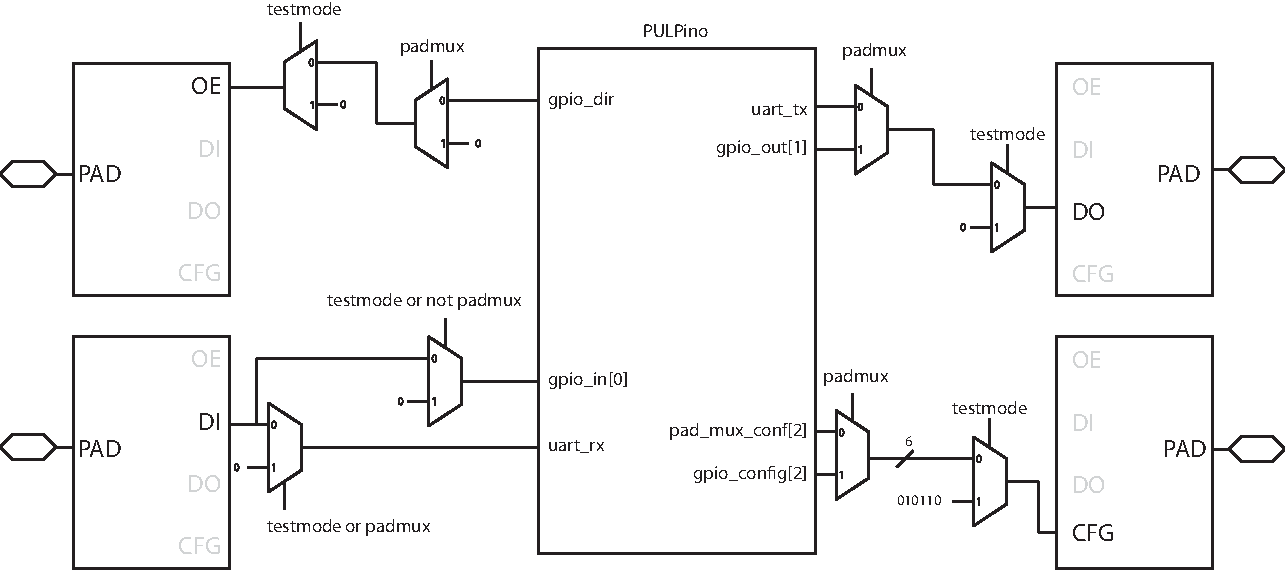
\includegraphics[width=\linewidth]{./figures/pad_muxes}
  \caption{Multiplexed Pads}
  \label{fig:pad_muxes}
\end{figure}


\section{Verification}

\subsection{Functional}
% Do not forget to include information about how you managed to do the
% functional verification (golden model, testbench,
% etc.). Figure~\ref{fig:func_ver} illustrates an example setup.

% \begin{figure}[tb]
%   \centering
%   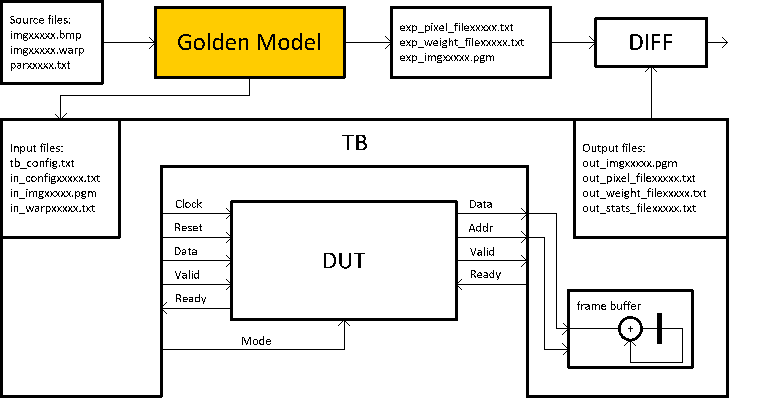
\includegraphics[width=\linewidth]{./figures/tb}
%   \caption{Functional verification setup.}
%   \label{fig:func_ver}
% \end{figure}

\subsection{Design for Testability (DFT)}

The RAM's input is bypassed in test mode in order to enable scan testing the combinatorial logic around the RAM. This is especially important for the RAM2AXI interfaces which allow operations on the bare memory. Furthermore, in order to observe the address pins of the RAM observation registers for the RAM address port have been added. The area overhead is small since Synopsys uses some sophisticated techniques to, on the one hand reuse the observation registers for both the instruction and the data RAM and on the other hand, only a few registers are necessary to make the signals of interest observable. \\
The memories itself will be tested with direct access through the JTAG interface. \\
The FLL has a dedicated DFT structure featuring a ScanEnable, ScanIn and ScanOut port. Until now the FLL is not part of one of the scan chains. \\
The current DFT numbers are related to post synthesis netlists. In a first run, a couple of weeks ago, I was able to achieve a bit more than 99 \% test coverage. While in the latest runs, most probably related to the newly instantiated pad frame and the FLL, test coverage deteriorated a bit and I am at 97\% for the current design. \\


\begin{lstlisting}
     Uncollapsed Stuck Fault Summary Report
 -----------------------------------------------
 fault class                     code   #faults
 ------------------------------  ----  ---------
 Detected                         DT     351339
 Possibly detected                PT         68
 Undetectable                     UD       1267
 ATPG untestable                  AU       8065
 Not detected                     ND         99
 -----------------------------------------------
 total faults                            360838
 test coverage                            97.72%
 fault coverage                           97.38%
 -----------------------------------------------
\end{lstlisting}

\subsubsection{Automated Testpattern Generation}

\section{Area}

On the final design there is approximately 25\% core area left (on a ninth module). Detailed area results are listed in figure~\ref{fig:area}. Note that the RAMs are no longer listed as a separate design entry as they are completely ungrouped for better synthesis results. Pad instances do not show up as seperate design entries since they are not over 1 kGE alone, but accumulated they are a significant part of the overall area.

% ------- Python generated ---------
\begin{figure}[ht!]
\centering
\begin{tabularx}{\textwidth}{Xllllll}
\textbf{Entity} &  \multicolumn{3}{l}{\textbf{Total Cells (kGE)}}  &  \multicolumn{3}{l}{\textbf{\% Total}}  \\\hline
imperio&700&&&100.0&&\\
pulpino\_i&500&&&73.1&&\\
$\quad$axi\_interconnect\_i&&6&&&1.0&\\
$\quad\quad$axi\_node\_i&&&6&&&1.0\\
$\quad\quad$others &&&0&&&0\\
$\quad$clk\_rst\_gen\_i&&12&&&1.8&\\
$\quad\quad$others &&&0&&&0.0\\
$\quad$core\_region\_i&&400&&&63.6&\\
$\quad\quad$RISCV\_CORE&&&40&&&5.8\\
$\quad\quad$adv\_dbg\_if\_i&&&5&&&0.8\\
$\quad\quad$axi\_slice\_core2axi&&&2&&&0.4\\
$\quad\quad$data\_mem\_axi\_if&&&5&&&0.8\\
$\quad\quad$instr\_mem\_axi\_if&&&5&&&0.8\\
$\quad\quad$others &&&0&&&0.0\\
$\quad$peripherals\_i&&50&&&6.8&\\
$\quad\quad$apb\_event\_unit\_i&&&3&&&0.5\\
$\quad\quad$apb\_gpio\_i&&&3&&&0.5\\
$\quad\quad$apb\_i2c\_i&&&1&&&0.2\\
$\quad\quad$apb\_pulpino\_i&&&2&&&0.3\\
$\quad\quad$apb\_spi\_master\_i&&&8&&&1.2\\
$\quad\quad$apb\_timer\_i&&&3&&&0.5\\
$\quad\quad$axi2apb\_i&&&1&&&0.2\\
$\quad\quad$axi\_spi\_slave\_i&&&8&&&1.3\\
$\quad\quad$i\_apb\_uart&&&14&&&2.1\\
$\quad\quad$others &&&0&&&0.0\\
\end{tabularx}
\caption{Area estimates (UMC65 - LVT 1.2V) @ 1.3ns - 1 GE = 1.44 \textmu m$^2$}
\label{fig:area}
\end{figure}
% ------- Python generated ---------

\begin{figure}[tb]
  \centering
  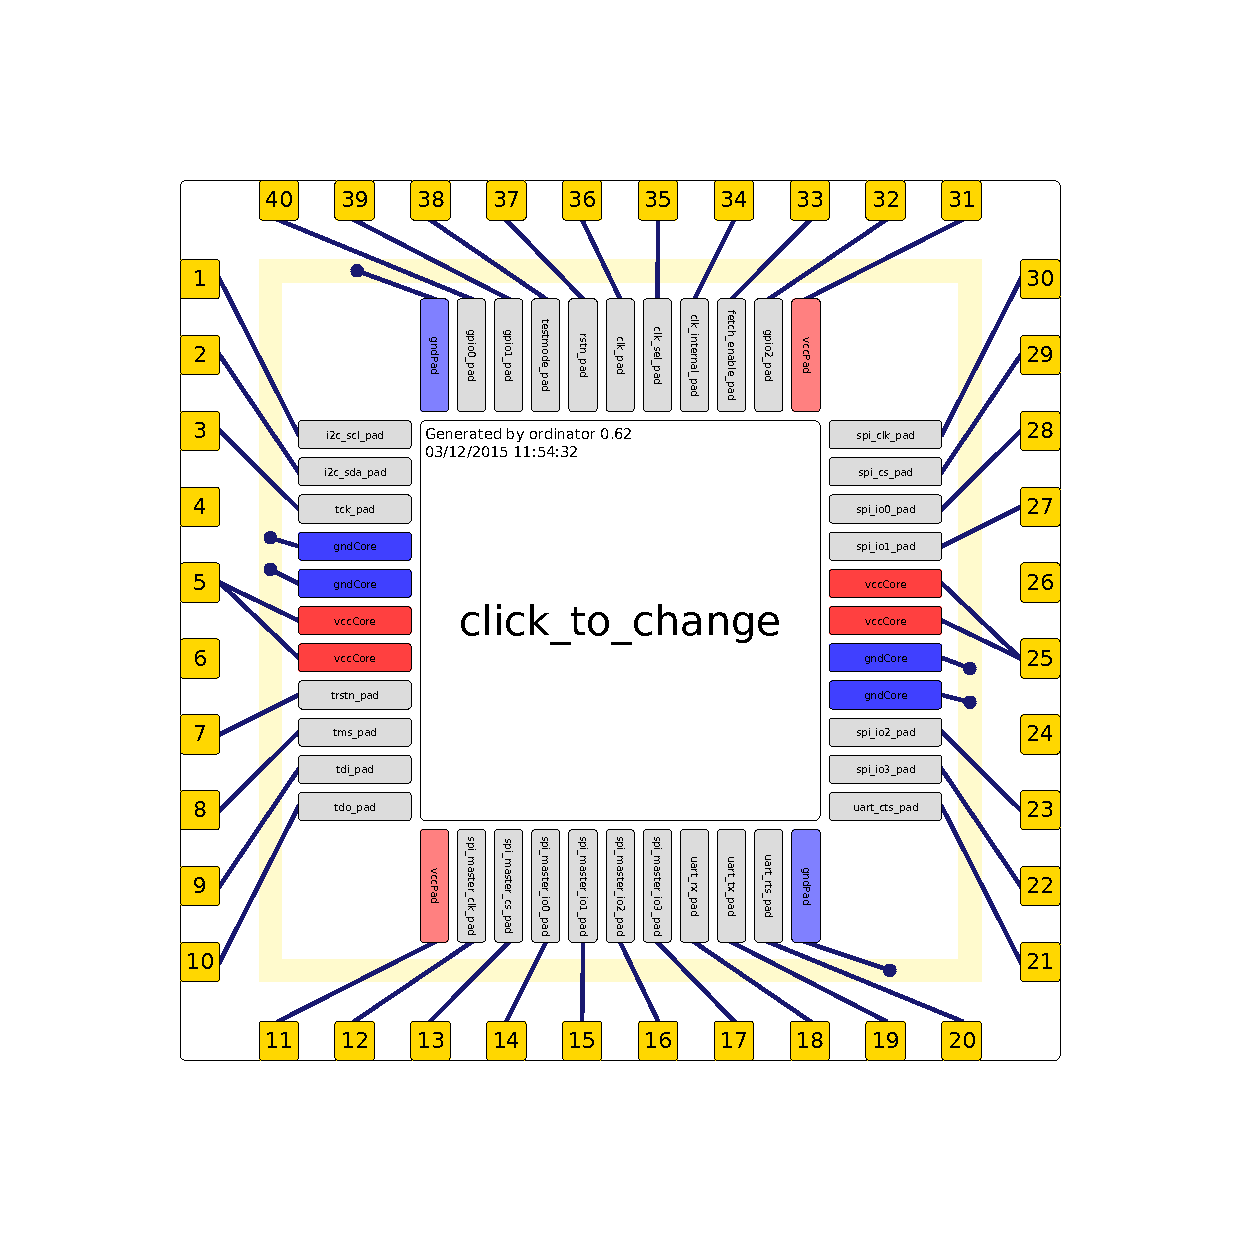
\includegraphics[width=\linewidth]{./figures/pad_instaces_img_ord}
  \caption{Bonding diagram}
  \label{fig:bonding_diagram}
\end{figure}

\section{Timing}

%talk about timing and how timing closure was achieved.

\section{Power}

Lowering power has always been a key driving factor for the PULP group. As a matter of fact power consumption has been a point of interest for \pulpino as well.

In order to estimate power consumption I extended the current testbench to automatically trigger ModelSims VCD dumps. Additionally I configured the CMake environment (for more information you may want to check the Getting Started Guide~\ref{sec:getting_started}) to have a distinct power target. This makes it particularly easy to run a power estimation.

For the time being I conducted three different measurements that are mostly representative for Imperio's application context.

\begin{enumerate}
    \item Interrupt Test: The core is clock gated most of the time in this scenario. It is woken up periodically and performs an UART transaction when it wakes up.
    \item Hello World: Trivial UART output. The core is not put to a particular low power state. Most of the operations are memory operations (instruction and data fetches).
    \item Matrix Multiplication: Computational intensive operation. The core needs to fetch a lot of data from the memories and performing computational costly operations, like multiplications and additions on it. This case should be representative for high density computation. 
\end{enumerate}

Power consumption can be split up into the following three components~\cite{Kaeslin08}:
\begin{itemize}
    \item Internal power $P_{int}$: power dissipated for charging and discharging the cell's internal capacitances.
    \item Switching power $P_{ext}$: this amounts to the power that gets dissipated for charging external load capacitances (input capacitance of driven cell plus wire capacitances) that are connected to the cell's output(s).
    \item Leakage power $P_{leak}$: power dissipated by the cell in absence of switching activity.
\end{itemize}
The total power dissipated by the circuit is the sum of these:
\[
    P_{tot} = P_{int} + P_{ext} + P_{leak}
\]
All power simulations where performed at 500 MHz, 1.2 V and 25 \textdegree C. Detailed results are depicted in table~\ref{tab:power}.

\begin{table}[htbp]
 \caption{Power Results (UMC65 - LVT 1.2V) @ 2ns, 25 \textdegree C}
 \label{tab:power}
\begin{tabularx}{\textwidth}{|X||l|l||l|l||l|l||l|}
  \hline
  \textbf{Test} & $P_{int}$& \% & $P_{ext}$ &  \% & $P_{leak}$ &  \% & $P_{tot}$\\ \hline
Interrupt Test & 7.10 & 57.84 & 5.00 &  40.64 & 0.17 & 1.52 & 12.28 \\ \hline
Hello World & 19.80 & 59.64 & 13.25 & 39.88 & 0.19 & 0.56 & 33.23 \\ \hline
Mat. Mul. & 32.00 & 60.00 & 21.17 & 39.68 & 0.19 & 0.35 & 53.35 \\ \hline
  \end{tabularx}
  \end{table}
% \section{Results}


% If you only have very few results, it might be a better approach to
% insert them into this chapter (instead of putting the results into a
% separate one).


